\documentclass[12pt, letterpaper]{article}
\usepackage{setspace}
\usepackage[spanish,mexico]{babel}                                  % Mexican spanish language
\usepackage[utf8]{inputenc}                                         % Input accented chars
\usepackage[T1]{fontenc}                                            % Allows to copy accented chars
\usepackage[top=1in, bottom=1in, left=1in, right=1in]{geometry}     % Margins
\usepackage{palatino}                                               % Use the Palatino font by default
\usepackage{mathtools}                                              % Tools form mathematics

\doublespacing

\begin{document}

\title{Conversión de coordenadas}
\author{Eduardo Jiménez Hernández}
\date{\today}
\maketitle

\section{Introducción}

El programa \textbf{Coordinates Conversion Tool} es una herramienta de cómputo que tiene la finalidad de ayudar al usuario a realizar los cálculos necesarios para la conversión entre coordenadas geográficas y la proyección Universal Transversa de Mercator (UTM).

Este documento indica el uso recomendado del programa bajo sistemas operativos Windows 10\textsuperscript{\textregistered} y Unix-like (macOS, GNU/Linux).

\section{Instalación}

\subsection{Windows}

La instalación del programa se realiza simplemente haciendo clic en el archivo llamado \textbf{Setup.exe} y siguiendo las instrucciones que aparecen en la pantalla.

\subsection{Unix-like}

Por el momento no se proporcionan binarios para sistemas operativos tipo Unix (macOS, GNU/Linux), y debido a esto se debe compilar el código fuente que fue creado usando Qt 5.8.

\section{Descripción}

Para iniciar el programa haga clic en el ícono creado en el Menú de inicio o en el Escritorio del sistema. Aparecerá una ventana como la siguiente:

\begin{figure}[h]
    \centering
    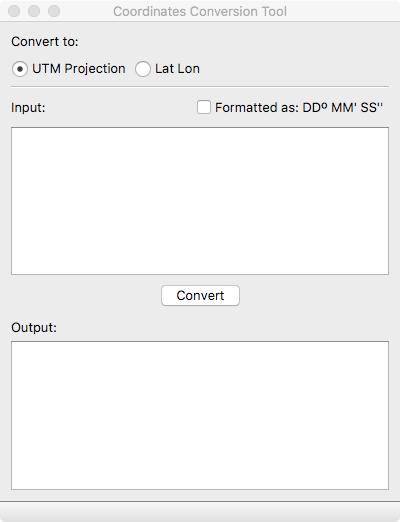
\includegraphics[width=0.5\textwidth]{img/mainwindow.png}
    \caption{Ventana principal.}
    \label{fig:mainwindow}
\end{figure}

Por el momento el programa se encuentra únicamente en idioma inglés, por lo que se hará una breve descripción de su funcionamiento.

\clearpage

\section{Conversión de coordenadas}

La conversión de coordenadas geográficas a UTM se hace de la siguiente forma:

\begin{figure}[h]
    \centering
    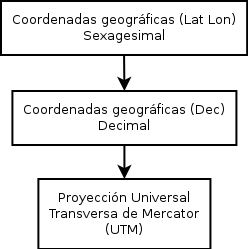
\includegraphics[width=0.35\textwidth]{img/geo2utm.png}
    \caption{Conversión de coordenadas geográficas (Lat Lon) a UTM.}
    \label{fig:geo2utm}
\end{figure}

Y el procedimiento inverso es:

\begin{figure}[h]
    \centering
    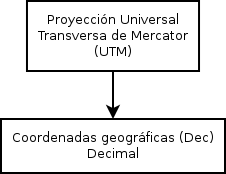
\includegraphics[width=0.35\textwidth]{img/utm2geo.png}
    \caption{Conversión de UTM a coordenadas geográficas (Lat Lon).}
    \label{fig:utm2geo}
\end{figure}

El programa puede convertir un par de coordenadas o una lista de varias coordenadas, antes de ver como se hace una conversión es necesario conocer los tipos de coordenadas.


\subsection{Formatos de coordenadas}


Las coordenadas Geográficas son ángulos, que representan latitud y longitud, generalmente se expresan de dos formas:

\begin{enumerate}
\item \textbf{Notación Sexagesimal} (de base 60): las coordenadas se expresan en grados ($º$), minutos ($'$) y segundos ($''$). Los segundos pueden tener partes decimales. La expresión GG MM SS es una forma de escribir grados, minutos y segundos. Ejemplos:

$12º34'34''$

$124º45'34.70''$

\item \textbf{Notación Decimal} (de base 10): las coordenadas se expresan únicamente en grados ($º$) quedando los minutos y segundos dentro de la parte decimal (GG.GG). Ejemplos:

$23.2345º$

$123.696º$

\end{enumerate}

Finalmente las coordenadas UTM representan las posiciones X, Y en un plano divido en husos o zonas. Por ello las coordenadas UTM requieren de tres elementos:

\begin{itemize}
\item Coordenada X, 
\item Coordenada Y, 
\item Zona UTM (Huso).
\end{itemize}

\textbf{NOTA:} Cada huso tiene asignado un meridiano central, que es donde se sitúa el origen de coordenadas. La coordenada X es relativa a este meridiano central por ello es importante conocer la zona en la que se encuentra.

\section{Hacer una conversión simple}

\subsection{Entrada de datos}

\begin{enumerate}
\item Seleccionar el tipo de conversión. En la parte superior de la aplicación se puede leer el texto \textbf{Convertir a} (``Convert to:'') Si se tienen coordenadas geográficas y se quieren convertir a UTM hay que seleccionar la opción \textbf{UTM projection}. En caso de que las coordenadas estén en formato sexagesimal (Grados, minutos y segundos), se debe marcar la opción \textbf{Formatted as DDMMSS}. Por el contrario si las coordenadas están en la proyección UTM y se desea pasarlas a geográficas se debe seleccionar la opción (``Convert to:'') \textbf{Lat Lon}.

\item Introducir las coordenadas.
	\begin{enumerate}
	\item Manualmente. Para hacer una conversión simple solo hay que escribir las coordenadas (con el formato correcto) en el campo de la parte superior (``Input'').
	\item También es posible abrir un archivo de texto delimitado con las coordenadas que se desea convertir en el formato mostrado en la figura y el texto aparecerá en el campo de entrada (``Input''). Para usar esta opción se debe usar el menú \textbf{File > Open file}.
	
	\begin{figure}[h]
	    \centering
	    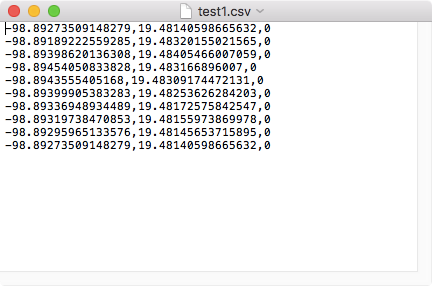
\includegraphics[width=0.5\textwidth]{img/textfile.png}
	    \caption{Formato de archivo de texto.}
	    \label{fig:textfile}
	\end{figure}
	
	\end{enumerate}
\end{enumerate}

Es importante mencionar que en cualquier caso se deben separar las coordenadas por una coma (o el delimitador seleccionado) y colocar en la primer columna la longitud o la coordenada X, seguido de la latitud o la coordenada Y. En la tercera columna se debe colocar la zona UTM cuando se introduzcan coordenadas en esta proyección.

\subsection{Convertir}

Una vez que la entrada de datos se ha hecho correctamente solo hay que dar clic en el botón para hacer la conversión. Las coordenadas convertidas aparecerán en el campo de texto inferior (``Output''), como se muestra en la figura.

\begin{figure}[h]
    \centering
    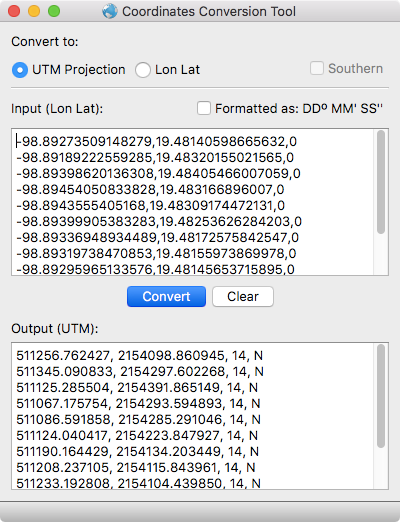
\includegraphics[width=0.5\textwidth]{img/conversion.png}
    \caption{Conversión de coordenadas.}
    \label{fig:conversion}
\end{figure}

Los resultados se pueden copiar o guardar según se requiera por el usuario.

\subsection{Otras opciones}

\begin{itemize}
\item \textbf{Seleccionar el delimitador.} El programa soporta texto delimitado por comas, espacios y tabulaciones, por omisión se utiliza comas. Para cambiarlo solo hay que seleccionar el necesario en el menú \textbf{Options > Delimiter} antes de hacer la conversión.
\item \textbf{Seleccionar el dátum.} Por el momento el programa soporta dos dátums: Hayford y WGS84, por omisión se utiliza el segundo. Para cambiarlo se debe usar el menú \textbf{Options > Datum}.

\end{itemize}
\end{document}